\documentclass[twoside,10pt]{article}
\usepackage{/Users/bradenhoagland/latex/styles/toggles}
%\toggletrue{sectionbreaks}
%\toggletrue{sectionheaders}
\newcommand{\docTitle}{HW 2}
\usepackage{/Users/bradenhoagland/latex/styles/common}
\importStyles{modern}{rainbow}{boxy}

%\renewcommand{\theenumi}{\alph{enumi}}

\begin{document}
%\tableofcontents

%--------------------------------------------------------------------------------
% 1
%--------------------------------------------------------------------------------
\begin{exer}[Lesson 3, 5 points]
	Compute $\beta_0$ and $\beta_1$ of the graphs $G_1$ and $G_2$ given in the Lesson 3 notes.
\end{exer}

\[
\begin{tikzcd}
                                           & G_1                                        &     &                                           & G_2                    &     \\
                                           & v_4 \arrow[r, no head]                     & v_5 &                                           &                        & v_5 \\
v_3 \arrow[ru, no head] \arrow[d, no head] &                                            &     & v_3 \arrow[r, no head] \arrow[d, no head] & v_4 \arrow[d, no head] &     \\
v_1                                        & v_2 \arrow[lu, no head] \arrow[l, no head] &     & v_1                                       & v_2 \arrow[l, no head] &    
\end{tikzcd}
\] 

Since our simplices are both 1-dimensional, our chain complex in both cases will be
\[
\begin{tikzcd}
	0 \rar{\p_2} & C_1 \rar{\p_1} & C_0 \rar{\p_0} & 0,
\end{tikzcd}
\] so the homology groups will be
\begin{align*}
	H_0 &= \frac{\ker \p_0}{\im \p_1} \cong \frac{C_0}{\im \p_1}, \\
	H_1 &= \frac{\ker \p_1}{\im \p_0} \cong \ker \p_1.
\end{align*}
For our two graphs $G_1$ and $G_2$, we have $\dim C_0 = \dim C_1 = 5$ since each graph has 5 vertices and 5 edges each. Thus the betti numbers are
\begin{align*}
	\beta_0 &= \dim H_0 \\
		&= \dim C_0 - \dim (\im \p_1) \\
		&= \dim C_0 -(\dim C_1 - \dim (\ker \p_1)) \\
		&= \dim (\ker \p_1)
		\intertext{and}
	\beta_1 &= \dim(\ker \p_1).
\end{align*}
So both these graphs 0th and 1st betti numbers are both just the dimension of the kernel of $\p_1$. We compute these kernels below.

\begin{enumerate}
	\item For $G_1$, an element of the kernel of $\p_1$ satisfies
		\begin{align*}
			\p_1\left( \alpha[v_1,v_2]+\beta[v_2,v_3]+\gamma[v_1,v_3]+\delta[v_3,v_4]+\varepsilon[v_4,v_5] \right) &= 0 \\
			\alpha(v_1+v_2) + \beta(v_2+v_3)+\gamma(v_1+v_3)+\delta(v_3+v_4)+\varepsilon(v_4+v_5) &= 0 \\
			(\alpha+\gamma)v_1 +(\alpha+\beta)v_2+(\beta+\gamma+\delta)v_3+(\delta+\varepsilon)v_4+\varepsilon v_5 &= 0.
		\end{align*}
		Each coefficient must then be zero, giving us a system that we can represent in matrix form. Performing Gaussian elimination gives
		\[
		\begin{pmatrix}
			1 & 0 & 1 & 0 & 0 \\
			1 & 1 & 0 & 0 & 0 \\
			0 & 1 & 1 & 1 & 0 \\
			0 & 0 & 0 & 1 & 1 \\
			0 & 0 & 0 & 0 & 1
		\end{pmatrix}
		\leadsto
		\begin{pmatrix}
                        1 & 0 & 1 & 0 & 0 \\
                        0 & 1 & 1 & 0 & 0 \\
                        0 & 0 & 0 & 1 & 0 \\
                        0 & 0 & 0 & 0 & 1 \\
                        0 & 0 & 0 & 0 & 0
                \end{pmatrix},
	\] so $\delta = \varepsilon = 0$ and $\alpha=\beta=\gamma$. The space of all viable tuples $(\alpha,\beta,\gamma,\delta,\varepsilon)$ is then spanned by $(1, 1, 1, 0, 0)\gamma$ (the single triangle in the diagram), so $\dim(\ker p_1) = 1$. Thus $\beta_0=\beta_1 = 1$.

	\item For $G_2$, we can similarly derive that any element of the kernel of $\p_1$ satisfies
		\begin{align*}
			\p_1\left( \alpha[v_1,v_2]+\beta[v_2,v_4]+\gamma[v_1,v_4]+\delta[v_1,v_3]+\varepsilon[v_3,v_4] \right) &= 0 \\
			(\alpha+\gamma+\delta)v_1+(\alpha+\beta)v_2+(\delta+\varepsilon)v_3+(\beta+\gamma+\varepsilon)v_4 &= 0.
		\end{align*}
		Once again, we perform Gaussian elimination on the matrix form of this system to get
	\[
                \begin{pmatrix}
                        1 & 0 & 1 & 1 & 0 \\
                        1 & 1 & 0 & 0 & 0 \\
                        0 & 0 & 0 & 1 & 1 \\
                        0 & 1 & 1 & 0 & 1 \\
                \end{pmatrix}
                \leadsto
                \begin{pmatrix}
                        1 & 0 & 1 & 1 & 0 \\
                        0 & 1 & 1 & 1 & 0 \\
                        0 & 0 & 0 & 1 & 1 \\
                        0 & 0 & 0 & 0 & 0 \\
		\end{pmatrix},
	\] so $\alpha=\beta=\gamma+\delta$ and $\delta=\varepsilon$. Then the whole space of viable $(\alpha,\beta,\gamma,\delta,\varepsilon)$ is spanned by $(1,1,1,0,0)\gamma + (1,1,0,1,1)\delta$, the square and one of the triangles in the diagram. Thus $\dim (\ker \p_1) = 2$, so $\beta_0=\beta_1=2$.
\end{enumerate}




\newpage

%--------------------------------------------------------------------------------
% 2
%--------------------------------------------------------------------------------
\begin{exer}[Lesson 4, 5 points]
	Compute the zero dimensional persistence diagram of the filtered graph (i.e. graph and associated monotonic function) shown in the Lesson 4 notes.
\end{exer}

\[
\begin{tikzcd}
1 \arrow[d, "6"', no head] & 2 \arrow[r, "3", no head] \arrow[d, "7"', no head] & 3 \\
4                          & 5                                                  &  
\end{tikzcd}
\] 

The persistence diagram is below.
\begin{figure}[H]
	\centering
	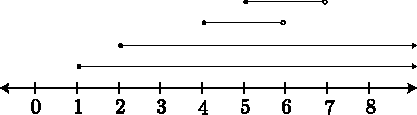
\includegraphics[scale=1]{fig/persistent.pdf}
	%\caption{}
\end{figure}
As a set, this is
\[
	\left\{ [1,\infty), [2,\infty), [4,6), [5,7) \right\}.
\] 


\end{document}
